% -*- coding: utf-8 -*-
% !TEX encoding = UTF-8 Unicode
% !TEX root =  main.tex




\chapter{Einleitung}
\label{chap:Zielsetzung}

Am Institut für Systemtechnik der Hochschule Bochum werden im Bereich der elektrischen Antriebstechnik und Leistungselektronik Praktika von Studierenden geleistet, welche zur Aus- und Weiterbildung in dem jeweiligen Fachgebiet dienen.\\

Ziel dieses Projektes ist die Bestimmung und Anzeige des Polradwinkels einer Synchronmaschine, zur Verwendung in o.g. Praktika.
Die zahlreiche Erwähnung in Literatur und Vorlesung, bei gleichzeitig fehlender visueller Darstellung unter verschiedenen Belastungsfällen, motiviert dieses Projekt. \cite{schroeder,albach,bergmann}\\

Das vorhandene und vom Auftraggeber bereitgestellte UniTrain-System  \cite{unitrain} von Lucas Nülle dient dabei als Umgebung für die Praktika und stellt den Synchronmotor bereit, welcher in diesem Projekt untersucht werden soll.

\chapter{Grundlagen zur Synchronmaschine}

\section{Dreiphasensystem und Drehfeld}

Die Synchronmaschine ist ein elektrischer Antrieb, in welcher der Rotor synchron mit dem durch die Netzfrequenz vorgegebenen Drehfeld des Stators läuft. Im Gegensatz zu Asynchronmaschinen benötigen Synchronmaschinen eine magnetische Erregung des Läufers, wie z.B. einen als Permanentmagneten ausgeführten Rotor. Ein räumlich um eine Achse drehendes Magnetfeld wird in der Elektrotechnik als Drehfeld bezeichnet. Dieses Drehfeld wird mithilfe eines Dreiphasensystems erzeugt.
Ein Dreiphasensystem besteht aus drei sinusförmigen Wechselspannungen bzw. Wechselströmen, welche zueinander um \(120^\circ\) phasenverschoben sind. \cite{schroeder,	weissgerber}

\begin{align*}
u_1(t) &= \hat{u}\cdot \cos(\omega\:t+\varphi_1) \text{ mit } \varphi_1 = 0\\
u_2(t) &= \hat{u}\cdot \cos(\omega\:t+\varphi_2) \text{ mit } \varphi_2 = \frac{2}{3\pi}\\
u_3(t) &= \hat{u}\cdot \cos(\omega\:t+\varphi_3) \text{ mit } \varphi_3 =\frac{4}{3\pi}
\end{align*}

%\[u_3(t) = \hat{u}\cdot \cos(\omega\:t+\varphi_3) \text{ mit } \varphi_3 = 240^\circ\]


\begin{figure}[H]
	\centering
	\includegraphics[width=0.8\textwidth]{Bilder/Dreiphasensystem4} %70%
	\caption{Dreiphasensystem }
	\label{fig: Dreiphasensystem}
%	\caption*{Quelle: Eigene Darstellung}
\end{figure}

Betreibt man drei gleich gestaltete Spulen mit den zeitlich versetzten Spannungen und macht eine vereinfachte Betrachtung des Feldverlaufs in eben jenen Spulen, so kann man folgende Beobachtungen machen:

\begin{figure}[H]
	\centering
	\includegraphics[width=0.5\textwidth]{Bilder/verinfachtesFeld.png} %70%
	\caption{Vereinfachte Darstellung des Feldverlaufs \cite{albach}\\}
	\label{fig: Fluss Spule}
	%\caption*{Quelle: Albach, Grundlagen Elektrotechnik, Pearson}
\end{figure}


\begin{figure}[H]
	\centering
	\includegraphics[width=0.5\textwidth]{Bilder/zeiger.png} %70%
	\caption{Zeigerbild von zeitlich versetzten Feldern \cite{albach}\\}
	\label{fig: Fluss Spule}
	%\caption*{Quelle: Albach, Grundlagen Elektrotechnik, Pearson}
\end{figure}

Um ein Drehfeld zu erzeugen,werden die Spulen nun um \(120^\circ\) räumlich versetzt (Abb. 2.3). Mit diesen Voraussetzungen und der vereinfachten Betrachtung des Feldverlaufs in einer Spule, entsteht nun ein Feld mit konstantem Betrag und konstanter, netzabhängiger Winkelgeschwindigkeit (Abb. 2.4). Dies führt wiederum bei symmetrischer Belastung zu einer konstanten Leistungsabgabe und somit zu einer gleichbleibenden Belastung eines Generators bzw. eines elektrischen Antriebs. \cite{weissgerber}

\begin{figure}[H]
	\centering
	\includegraphics[width=0.7\textwidth]{Bilder/Drehfeld.png} %70%
	\caption{Resultierendes Drehfeld \cite{albach}\\}
	\label{fig: Drehfeld}
	%\caption*{Quelle: Albach, Grundlagen Elektrotechnik, Pearson}
\end{figure}


\section{Polradwinkel}


Als Polradwinkel bezeichnet man den Versatz zwischen Drehfeld und Polrad. Der Versatz wird durch mechanische Einflüsse wie z.B. Reibmomente und Lastmomente hervorgerufen. Grundsätzlich unterscheidet man beim Polradwinkel unter voreilenden (Generatorbetrieb) und nacheilenden (Motorbetrieb) Polrad.\cite{schroeder}

\begin{figure}[H]
	\centering
	\includegraphics[width=0.7\textwidth]{Bilder/polradwinkel2.png} %70%
	\caption{Beispiel für Polradwinkel im Motorbetrieb \cite{elektronikkurs}\\}
	\label{fig: Beispiele für Polradwinkel}
	%	\caption*{Quelle: http://elektronik-kurs.net/synchronmotoren-im-ein-und-mehrphasenbetrieb, 04.01.2019}
\end{figure}


Eine weitere Eigenschaft von Synchronmaschinen besteht bei der Ausführung des Läufers, z.B. als Schenkelpolmaschine oder Vollpolmaschine.\cite{schroeder,binder}

\begin{figure}[H]
	\centering
	\includegraphics[width=0.7\textwidth]{Bilder/schenkelpolmaschine.png} %70%
	\caption{Synchron-Schenkelpolmaschine \cite{schroeder}\\}
	\label{fig: Synchron-Schenkelpolmaschine }
\end{figure}

Der in Abb. 2.6 gezeigte Rotor, weist eine unterschiedliche Feldausbreitung des Statorfeldes in d- und q-Richtung auf. Dies folgt durch die unterschiedlich großen Luftspalte in d- und q-Achse. Dieses Verhalten wird auch als anisotrop
bezeichnet.\cite{schroeder,binder}

\begin{figure}[H]
	\centering
	\includegraphics[width=0.7\textwidth]{Bilder/vollpolmaschine.png} %70%
	\caption{Synchron-Vollpolmaschine \cite{schroeder}\\}
	\label{fig: Synchron-Vollpolmaschine }
\end{figure}

Ist bei der in Abb. 2.7 gezeigte Vollpolmaschine der Rotor konstruktiv Rotationssymmetrisch aufgebaut, so wird nicht mehr zwischen Induktivitäten in d- und q-Achse unterschieden, da sich die Feldausbreitung des Statorfeldes in d- und q-Richtung gleich verhält.\cite{schroeder} Dieses Verhalten wird deshalb als isotrop bezeichnet.\cite{binder} \newline
Ein symmetrischer, als Permanentmagnet ausgeführter Rotor weist das Verhalten einer Synchron-Vollpolmaschine auf.\cite{schroeder} \newline
 Bei steigender mechanischer Last vergrößert sich der Polradwinkel bis zur maximalen Drehmomentabgabe, auch Kippmoment genannt. Dieser Arbeitspunkt wird für eine Maschine mit o.g. isotropen Verhalten bei einen Polradwinkel von $\vartheta = 90^\circ$ erreicht.\cite{schroeder,binder} Für eine Synchronmaschine mit ferromagneten ausgeführten Rotor und anisotropen Verhalten liegt dieser Arbeitspunkt zwischen $\vartheta = 45^\circ$.. $90^\circ$.\cite{binder}, da sich in der Schenkelpolmaschine, wie in Abb. 2.8 zu sehen ist, das Drehmoment und Reluktanzmoment addieren.
 
 
 \begin{figure}[H]
 	\centering
 	\includegraphics[width=0.7\textwidth]{Bilder/vglmomente.png} %70%
 	\caption{Funktion des elektromagnetischen Drehmoments $Me(\vartheta)$
der Schenkelpolmaschine,
bezogen auf den Wert des
Kippmoments $M_{p0}$ der
vergleichbaren
Vollpol-Synchronmaschine \cite{binder}\\}
 	\label{fig: Vergleich der wirkenden Drehmomente }
 \end{figure}
 
 
Abb. 2.9 zeigt die Feldausbreitung für eine Synchronmaschine mit einem als Permanentmagnet ausgeführten Rotor und anisotropen Verhalten,
Das Feld des Stators magnetisiert die d-Achse des Rotors und muss daher die Magnete überqueren, die passiv wie Luft wirken, was zu einer verringerten d-Induktivität führt (linke Abbildung in Abb. 2.9). der Ständerfluss magnetisiert die q-Achse des Rotors und vermeidet daher weitgehend den Bereich der Magnete, was zu einer höheren q-Induktivität führt (rechte Abbildung in Abb.2.9).\cite{binder}

   
   \begin{figure}[H]
 	\centering
 	\includegraphics[width=0.7\textwidth]{Bilder/pesm.png} %70%
 	\caption{Schematische Darstellung eines 2-poligen Läufers mit eingebetteten Magneten \cite{binder}\\}
 	\label{fig: Vergrabene Magnete }
 \end{figure}
 
 Durch den in Abb. 2.9 gezeigte Rotor entsteht der sogenannte "inverse" Reluktanzeffekt, dieser hat zur Folge, dass das resultierende Kippmoment $M_{p0}$ für Polradwinkel $> 90^{\circ}$ erreicht wird.
 
  \begin{figure}[H]
 	\centering
 	\includegraphics[width=0.7\textwidth]{Bilder/vglmomente2.png} %70%
 	\caption{Funktion des elektromagnetischen Drehmoments $Me(\vartheta)$
 		der permanenterregten Synchronmaschine, setzt sich aus den synchronem Moment $M_{syn}$ und dem Reluktanzmoment $M_{rel}$ zusammen \cite{binder}\\}
 	\label{fig: Vergleich der wirkenden Drehmomente2 }
 \end{figure}
 
 
  Die untersuchte Synchronmaschine am UniTrain System besitzt einen als Permanentmagneten ausgeführten nicht eingebetteten Rotor und zeigt deshalb isotropes verhalten auf, da der Magnet passiv wie Luft wirkt. Der Rotor bleibt bei dem Arbeitspunkt $\vartheta = 90^\circ$ stehen und folgt für eine Netzfrequenz $>10\text{ }\si{\hertz}$ nicht mehr dem Drehfeld. 


\chapter{Konzeptionierung}

\section{Bestandsanalyse}

\subsection{UniTrain Interface}

Das UniTrain-System ist ein computergestütztes Trainings- und Experimentiersystem welches Theorie und Praxis vernetzt und somit den Studierenden auf dem entsprechenden Fachgebiet Kompetenzen vermitteln soll. An diesem System wird anschaulich die Funktionsweise von elektrischen Maschinen, wie z.B. der Synchronmaschine, vermittelt.\newline 
LabSoft ermöglicht den Zugriff auf interaktive Multimediakurse, sowie zur Steuerung der virtuellen Instrumenten, die zur Durchführung von Experimenten dienen \cite{labsoft, unitrain}. Das UniTrain-Sytem stellt ein Messinterface bereit, welches über analoge und digitale Mess- und Steuer- Ein / Ausgänge verfügt. Die Parameter der virtuellen Instrumente, wie z.B. Spannungsmessgerät, Spannungsquelle etc. lassen sich in LabSoft einstellen.\newline
 Labsoft muss auf einen externen Rechner installiert werden und über eine USB Schnittstelle mit dem UniTrain-System verbunden werden. 

\begin{figure}[H]
	\centering
	\includegraphics[width=0.9\textwidth]{Bilder/ganztollesdokument.pdf} %70%
	\caption{UniTrain Interface mit Experimentierkarte}
	\label{fig: UniTrain Interface mit Experimentierkarter}
\end{figure}

\subsection{NI myRio}


Die Datenerfassung und Datenverarbeitung erfolgt mit dem NI\footnote{National Instruments} myRio System von National-Instruments sowie der zugehören Software LabVIEW\footnote{Laboratory Virtual Instrumentation Engineering Workbench}, da diese Komponenten vom Auftraggeber vorgesehen wurden. Der NI myRio ist ein eingebettetes System, welches ursprünglich für Schulungszwecke entwickelt wurde.\cite{myrio}

\begin{figure}[H]
	\centering
	\includegraphics[width=0.5\textwidth]{Bilder/Ni-MyRio.jpg} %70%
	\caption{NI myRio \cite{myriobild}}
	\label{fig: NI myRio}
\end{figure}



Das Gerät verfügt über digitale sowie analoge Schnittstellen auf beiden Seiten des Geräts in Form von MXP\footnote{myRio Expansion Port}- und MSP\footnote{Mini System Port}-Anschlüssen. Die Klemmbelegung der Anschlüsse kann den Tabellen 3.1 und 3.2 entnommen werden. Der in diese Projekt verwendete NI myRio unterstützt auch eine W-LAN\footnote{Wireless Local Area Network}- Anbindung. Es besteht die Möglichkeit den NI myRio mit den Programmiersprachen C oder G zu programmieren.

\begin{table}[H]
	\centering
	\begin{tabular}{c|c|c}
		\hline
		Signal Name        &       Referenz        &           Beschreibung      \\ \hline
		+5V   & DGND &        $5\si{\volt}$ Ausgang      \\
		AI <0..3>   &     AGND   &       $0-5\si{ \volt}$ Analog Input      \\
		AO <0..1>   &     AGND   &       $0-5\si{ \volt}$ Analog Output      \\
		AGND   &     N/A   &       Referenz für Analog Input und Output      \\
		+3.3V  &     DGND &        $+3.3\si{\volt}$ Ausgang   \\
		DIO<0..15> &     DGND &        Digitaler Input und Output $3.3/5\si{ \volt}$  \\
		DGND&     N/A &       Referenz für Digitale $3.3/5\si{ \volt}$  Signale  \\
		\hline
	\end{tabular}
	\caption{Beschreibung der MXP Schnittstellen A und B}
	\label{tab:param_voltageDrop}
\end{table}


\begin{table}[H]
	\centering
	\begin{tabular}{c|c|c}
		\hline
		Signal Name       &       Referenz        &           Beschreibung      \\ \hline
		+15V/-15V  & AGND &        $+15/-15\si{ \volt}$ Ausgang      \\
		AI0+/AI0-   &     AGND   &    $+10/-10\si{ \volt}$  Analog Input      \\
		AI1+/AI1-   &     AGND   &      $+10/-10\si{ \volt}$  Analog Input      \\   
		AO <0..1>   &     AGND   &     $+10/-10\si{ \volt}$  Analog Output      \\
		AGND   &     N/A   &       Referenz für Analog Input und Output      \\
		+5V&     DGND &        $5\si{\volt}$ Ausgang    \\
		DIO<0..7> &     DGND &        Digitaler Input und Output $3.3/5\si{ \volt}$ \\
		DGND&     N/A &       Referenz für Digitale $3.3/5\si{ \volt}$ Signale  \\
		\hline
	\end{tabular}
	\caption{Beschreibung der MSP Schnittstellen C}
	\label{x}
\end{table}



\subsection{LabVIEW}

LabVIEW ist ein grafisches Programmiersystem von der Firma National Instruments. Hauptanwendungsgebiete von LabVIEW sind die Mess-, Regel- und Automatisierungstechnik. Die Programmierung erfolgt mit einer grafischen Programmiersprache, genannt G, nach dem Datenfluss-Modell.\newline
Die in LabVIEW erstellten Programme werden als VI's\footnote{Virtuelles Instrument} bezeichnet und beinhalten sowohl eine Programmieroberfläche bzw. Blockdiagramm, als auch eine Experimentierumgebung. Die Experimentierumgebung dient zur Visualisierung des auf der Programmieroberfläche erstellten Datenfluss und wird auch als Frontpanel bezeichnet. LabVIEW bietet Kompatibilität mit den in Kapitel 3.1.2 beschriebenen NI myRio und anderer NI Hardware.\cite{myrio}

\begin{figure}[H]
	\centering
	\includegraphics[width=0.7\textwidth]{Bilder/Datenflussbsp.png} %70%
	\caption{Beispiel für ein Datenflussmodell }
	\label{fig: Beispiel für ein Datenflussmodell}
\end{figure}

\begin{figure}[H]
	\centering
	\includegraphics[width=0.7\textwidth]{Bilder/Exp-Umgebung.png} %70%
	\caption{Beispiel für eine Experimentieroberfläche}
	\label{fig: Beispiel für eine Experimentieroberfläche}
\end{figure}

%hier kommt eine Tabelle mit den Spezifikationen hin\

\subsection{Surface Pro 4}

Das Surface Pro 4 ist ein Tablet PC 4. Generation der gleichnamigen Produktfamilie der Firma Microsoft. Für die Laborversuche wurde auf dem Surface Pro 4 LabVIEW installiert und in Verbindung mit dem NI myRio genutzt. Auf dem Tablet PC ist Windows 10 Pro installiert.

\begin{figure}[H]
	\centering
	\includegraphics[width=0.5\textwidth]{Bilder/surface-pro4.jpg} 
	\caption{Surface Pro 4 \cite{notebookcheck}\\}
	\label{fig: Surface}
	%\caption*{Quelle: https://www.notebookcheck.com/Microsoft-Surface-Pro-4-Core-i7.157262.0.html, 04.01.2019}
\end{figure}


\begin{table}[h]
	\centering
	\begin{tabular}{c|c|c}
		\hline
		Komponente & Typ & Eigenschaft\\ \hline
		CPU & i7-6650U & 2 x 2.20 - 3.40 GHz\\
		RAM& - & 8GB\\
		Speicher &     SSD  &    256 GB    \\
		Ports  &     -   &       USB 3.0, Mini DisplayPort, microSD     \\
		\hline
	\end{tabular}
	\caption{Spezifikation des Surface Pro 4}
	\label{x}
\end{table}

\subsection{Laborrechner}

Der Laborrechner ist ein Desktop PC und wurde für die Versuche am UniTrain System benutzt. Auf dem Laborrechner ist Windows 10 und Labsoft installiert und kann für zukünftige Anwendungsszenarien mit LabVIEW erweitert werden. Dadurch ist der in Kapitel 3.1.4 beschriebene Tablet PC nicht weiter von Nöten, da auch die Anzahl der benötigten Schnittstellen ausreichend ist.

\begin{figure}[H]
\centering
\includegraphics[width=0.5\textwidth]{Bilder/laborrechner.jpeg} 
\caption{Laborrechner}
\label{fig: laborrechner}
%\caption*{Quelle: Eigene Darstellung}
\end{figure}

\begin{table}[h]
	\centering
	\begin{tabular}{c|p{4cm}|p{4cm}}
		\hline
		Komponente & Typ & Eigenschaft\\ \hline
		CPU & i5-7600 & 4 x 3.5 GHz\\ \hline
		RAM& - & 16GB\\ \hline
		Speicher &     SSD  &    512 GB    \\\hline
		Ports  &     -   &       6 x USB 3.0,4 x USB 2.0, 2 x DisplayPort,1 x HDMI, 2 x VGA, 1 x Ethernet     \\
		\hline
	\end{tabular}
	\caption{Spezifikation des Laborrechners}
	\label{x}
\end{table}


\section{Anforderungserhebung}

Um das in der Einleitung beschriebene Ziel im entsprechenden Rahmen des Entwicklungsprojekts umzusetzen, wird der Projektumfang mit dem Auftraggeber in Form eines Lastenhefts erstellt. Desweiteren wird für die im Lastenheft beschriebenen Anforderungen ein Verifikationsplan ausgearbeitet (siehe Kapitel 5).\newline



\section{Laborversuche}

In diesem Abschnitt wird über Laborversuche berichtet, welche nötig waren um sich in die gegebenen Systeme (siehe Kapitel 3.1) einzuarbeiten und die im Lastenheft festgehaltenen Anforderung umzusetzen.

\subsection{Induktivität der Wicklungen}
\subsubsection{Ziel:}

Um den Polradwinkel einer Synchronmaschine anhand eines Zeigerbildes zu berechnen, benötigt man unter anderen die Induktivität bzw. die daraus resultierende Synchrone Reaktanz der Synchronmaschine.\cite{schroeder}
Da der Hersteller des UniTrain Systems keine Angaben über die Induktivität, sondern lediglich über den ohmschen Widerstand der Wicklungen gemacht hat, muss diese gemessen werden.


\subsubsection{Aufbau:}

\begin{figure}[H]
	\begin{center}
		\begin{tikzpicture}[circuit ee IEC, circuit symbol lines/.style={draw,thick}]
		
		%Matrix
		\def\spaltenabstand{1.5cm}
		\def\zeilenabstand{0.5cm}
		\def\zeilenzahl{9}
		\def\spaltenzahl{7}
		\foreach \i in {1,...,\zeilenzahl}
		\foreach \j in {1,...,\spaltenzahl}
		{
			\coordinate (S-\i-\j) at ({(\j-1)*\spaltenabstand},{-(\i-1)*\zeilenabstand});
			%\node at (S-\i-\j){+}; % Orientierungshilfe
		}
		
		%Schaltung
		\draw (S-2-1) to  [resistor={info=$R_i$}](S-4-1); 
		\draw (S-6-1) to  [inductor={info=$L$}](S-8-1); 
		%\draw (S-4-2)[fill=white] circle [radius=15pt];
		\node[draw,circle,minimum size=1cm,inner sep=0pt] at (S-5-2){$L CR$};
		%Leiterbahnen
		
		\draw 
		(S-2-1)--(S-1-1)--(S-1-2)--(S-4-2)
		(S-6-1)--(S-4-1)
		(S-8-1)--(S-9-1)--(S-9-2)--(S-6-2);
		
		
		Knotenpunkte, Klemmen (extra zeichnen, so keine Überschneidungen)
		\foreach \p in {S-1-1,S-9-1}
		\draw[fill=white] (\p) circle [radius=2pt];
		
		%\foreach \p in {S-4-2,S-2-3,S-2-4,S-4-5,S-6-3,S-6-4}
		%\draw[fill] (\p) circle [radius=2pt];
		
		\end{tikzpicture}
	\end{center}
	\centering
	\caption{Versuchsaufbau Messung der Induktivität}
	\label{fig:Versuchsaufbau Messung der Indktivität}
\end{figure}


\subsubsection{Durchführung:}

Für die Messung der Induktivität wird ein LCR-Messgerät, wie in Abb. 3.7 gezeigt, an eine der drei vorhandenen Spulen angeschlossen. Hierbei ist zu beachten, dass die zu messende Spule von der Schaltung getrennt ist, sodass lediglich die Induktivität der einzelnen Spule gemessen wird. Da allgemein angenommen wird, dass der Innenwiderstand und die Induktivität bei Spulen in Reihe geschaltet sind, wird die Einstellung $serial$ am LCR-Messgerät vorgenommen.

\subsubsection{Interpretation der Messergebnisse:}

Die Messung ergab eine Induktivität von $L=16 \text{ } \si{mH}$. Der daraus resultierende induktive Blindwiderstand ist im Bezug zum ohmschen Leiterwiderstand ($R=20\ohm$) vernachlässigbar klein. Dies hat zur Folge, dass die Phasenverschiebung, wie in Abb. 3.8 zu sehen, zwischen Strom und Spannung nicht wesentlich ist. Somit ist eine grafische Lösung zur Veranschaulichung und weiteren Berechnung, z.B. anhand eines Zeigerbildes, nicht möglich.


\begin{figure}[H]
	\centering
	\includegraphics[width=1.0\textwidth]{Bilder/vergleichphase.png} 
	\caption{Vergleich Strom und Spannung}
	%\caption*{Quelle: https://www.notebookcheck.com/Microsoft-Surface-Pro-4-Core-i7.157262.0.html, 04.01.2019}
\end{figure}




\subsection{Strommessung der Stränge und Berechnung des Raumzeigers der Drehfeldmaschine}
\subsubsection{Ziel:}
\label{sec:zielstrommessung}


Um Aussagen über das Drehfeld (siehe Kapitel 2.1) einer Synchronmaschine zu treffen benötigt man die entsprechenden Strangströme. Sind die drei Strangströme bekannt, kann man mithilfe einer Raumzeigertransformation die räumlichen und zeitlichen Zusammenhänge des Drehfelds darstellen.\cite{schroeder,binder}\newline
In diesem Versuch werden aufgrund der Hardwaregegebenheiten des NI myRIO's lediglich zwei der drei vorhandenen Strangströme gemessen, der dritte Strangstrom wird mithilfe der Kirchoffschen Knotengleichung berechnet.

\[i_1(t)+i_2(t)+i_3(t)=0\]


Um die Ströme zu messen, werden Widerstände, auch Shunts genannt, in Reihe zu den Wicklungen geschaltet. Die in diesem Versuch verwendeten Shunts weisen einen Widerstand von 1$\Omega$ auf. Die Spannungen über den Widerständen werden mithilfe der analogen Eingänge des NI myRio gemessen und anhand des Ohmschen Gesetzes zu Strömen umgerechnet. Die Analogeingänge sind in Abbildung 3.9 als Voltmeter abgebildet. Es werden bewusst drei Shunts benutzt, um eine symmetrische Belastung des Motors zu gewährleisten.
Um aus den Strangströmen Information über den Raumzeiger zu bekommen, wird eine Raumzeigertransformation durchgeführt.


\subsubsection{Aufbau:}


\begin{figure}[H]
	\begin{center}
		\begin{tikzpicture}[circuit ee IEC, circuit symbol lines/.style={draw,thick}]
		
		%Matrix
		\def\spaltenabstand{1.5cm}
		\def\zeilenabstand{0.5cm}
		\def\zeilenzahl{15}
		\def\spaltenzahl{7}
		\foreach \i in {1,...,\zeilenzahl}
		\foreach \j in {1,...,\spaltenzahl}
		{
			\coordinate (S-\i-\j) at ({(\j-1)*\spaltenabstand},{-(\i-1)*\zeilenabstand});
			%\node at (S-\i-\j){+}; % Orientierungshilfe
		}
		
		%Schaltung
		\draw (S-8-2) to  [resistor={info=$R_1$}](S-10-2); 
		\draw (S-12-2) to  [inductor={info=$L_1$}](S-14-2);
		
		\draw (S-8-3) to  [resistor={info=$R_2$}](S-10-3); 
		\draw (S-12-3) to  [inductor={info=$L_2$}](S-14-3);
		
		\draw (S-8-4) to  [resistor={info=$R_3$}](S-10-4); 
		\draw (S-12-4) to  [inductor={info=$L_3$}](S-14-4);
		
		
		%	\draw (S-12-5) to  [inductor={info=$L_3$}](S-14-5);
		
		%\draw (S-4-2)[fill=white] circle [radius=15pt];
		\node[draw,circle,minimum size=1cm,inner sep=0pt] at (S-9-1){$V$};
		\node[draw,circle,minimum size=1cm,inner sep=0pt] at (S-9-5){$V$};
		\node[] at (-0.5,-1.0) {V1};
		\node[] at (-0.5,-1.5) {V2};
		\node[] at (-0.5,-2.0) {V3};
		\node[] at (-0.5,-2.5) {COM};
		\node[] at (8.5,-3.6) {AGND};
		
	
		\node[draw, rotate=270, ground] at (7.5,-3.6){};
	    
		
		%Leiterbahnen
		
		\draw 
		(S-8-2)--(S-7-2)--(S-3-2)
		(S-12-2)--(S-10-2)
		(S-3-1)--(S-3-7)
		
		(S-8-3)--(S-7-3)--(S-4-3)
		(S-12-3)--(S-10-3)
		(S-4-1)--(S-4-7)
		
		(S-8-4)--(S-7-4)--(S-5-4)
		(S-12-4)--(S-10-4)
		(S-5-1)--(S-5-7)
		
		(S-6-1)--(S-6-7)
		(S-6-6)--(S-8-6)
		
		(S-7-2)--(S-7-1)--(S-8-1)
		
		(S-11-2)--(S-11-1)--(S-10-1)
		
		(S-7-4)--(S-7-5)--(S-8-5)
		
		(S-11-4)--(S-11-5)--(S-10-5)
		
		(S-14-2)--(S-15-2)--(S-15-3)--(S-14-3)
		(S-15-3)--(S-15-4)--(S-14-4);
		
		Knotenpunkte, Klemmen (extra zeichnen, so keine Überschneidungen)
		\foreach \p in {S-11-2,S-11-4,S-7-2,S-7-4}
		\draw[fill=white] (\p) circle [radius=2pt];
		
		\foreach \p in {S-15-3,S-3-2,S-4-3,S-5-4,S-6-6}
		\draw[fill] (\p) circle [radius=2pt];
		
		\end{tikzpicture}
	\end{center}
	\centering
	\caption{Schaltplan Versuch 2}
	\label{fig:Schaltplan Versuch 2}
%	\caption*{Quelle: Eigene Darstellung}
\end{figure}

\begin{align*}
R_1 &= R_2=R_3=R=1\Omega\\
L_1 &=L_2=L_3=L=16  \text{ }  \si{mH}\\
I_n	&=\frac{U_n}{R} \text{ mit } n =1,2,3
\end{align*}


\begin{figure}[H]
	\centering
	\includegraphics[width=0.6\textwidth]{Bilder/Unbenannt.png} %70%
	\caption{LabVIEW-Programm zur Erfassung der Shunt-Spannungen}
	\label{fig: Drehfeld}
%	\caption*{Quelle: Eigene Darstellung}
\end{figure}


In Abbildung 3.10 sieht man die Abtastung der beiden Strangströme, sowie die Berechnung des dritten Strangstroms. Das Abtasten erfolgt mithilfe einer While-Schleife, da die Analogeingänge bei einen neuen Iterationsschritt einen neuen Analogwert einlesen. Für weitere Analysen werden die abgetasteten Werte in einen Array gespeichert. Die Schleife hat eine Durchlaufzeit von 0.5 ms, daraus resultiert eine Abtastrate von 2 k$\si{\hertz}$. \cite{shiftregister,while,measure}

\subsubsection{Durchführung:}

Zur Durchführung muss in Labsoft die Spannungsquelle  \glqq Drehstromversorung\grqq{} ausgewählt und die gewünschten Parameter eingestellt werden.

\begin{figure}[H]
	\centering
	\includegraphics[width=0.4\textwidth]{Bilder/Drehstromquelle_Labsoft.png} %70%
	\caption{Spannungsquelle LabSoft}
	\label{fig: Spannungsquelle Labsoft}
%	\caption*{Quelle: Eigene Darstellung}
\end{figure}


Durch die Ausführung des entsprechenden LabVIEW VI, wie z.B. aus Abbildung 3.10, erhält man die gewünschten Messwerte und kann diese verarbeiten. Durch Aufbringen eines Drehmoments am Rotor, können verschiedene Lastfälle simuliert werden.


\subsubsection{Interpretation der Messergebnisse:}


Abbildung 3.12 zeigt die beiden gemessenen und den dritten berechneten Strangstrom, wobei wie zu erwarten drei um \(120^\circ\) phasenverschobene Ströme zu sehen sind.


\begin{figure}[H]
	\centering
	\includegraphics[width=0.6\textwidth]{Bilder/strom_gemessen.png} 
	\caption{Dreiphasensystem gemessen und berechnet}
	\label{fig: Dreiphasensystem gemessen und berechnet}
%	\caption*{Quelle: Eigene Darstellung}
\end{figure}


Die nun bekannten Strangströme können zu einen Raumzeiger zusammengefasst werden.

\begin{align*}
\vec{i}&=i_{\alpha}+ji_{\beta}=i_{1}+ai_{2}+a^{2}i_{3} \text{ mit } a = e^{j120^{\circ}}
\end{align*}

Durch Anwenden der komplexen Wechselstromrechnung erhält man die Form:

\begin{align*}
i_{\alpha}&=i_1-\dfrac{i_{2}-i_{3}}{2}\\
i_{\beta}&=\dfrac{i_{2}-i_{3}}{\sqrt{3}}\\
\vartheta&=\arctan \frac{i_{\beta}}{i_{\alpha}}
\end{align*}

Die einzelnen Komponenten wurden in Abb. 3.13 für alle Messwerte errechnet und geplottet. Mit entsprechenden Skalierungsfaktor wird der Stromzeiger aus Abb. 3.13 auch als Feldzeiger interpretiert. Das in der Abbildung gezeigte Drehfeld, weist die Struktur eines Hexagons auf. Die Versorgungsspannung der Synchronmaschine wird durch eine Pulsweitenmodulation im UniTrain Interface generiert, welche aufgrund der Raumzeigermodulation die Form des Drehfelds als Hexagon abbildet.\cite{leistungselektronik}

\begin{figure}[H]
	\centering
	\includegraphics[width=0.6\textwidth]{Bilder/Hexagon.png} %70%
	\caption{Drehfeld der Experimenters}
	\label{fig: Drehfeld der Experimenters}
	%\caption*{Quelle: Eigene Darstellung}
\end{figure}


\subsection{Erfassen des Rotors und Berechnung des Polradwinkels}

\subsubsection{Ziel:}


Um die Rotorposition zu erkennen wird der induktive Sensor IE5345 \cite{induktiverse} der Firma ifm benutzt. Aufgrund von folgenden Vorteilen im Vergleich zu anderen Sensoren, wie z.B. kapzitive oder optische Sensoren, wird die Nutzung des o.g. Sensors konkretisiert: 

\begin{itemize}
	\item Geringe Kosten
	\item Geringer Schaltabstand
	\item Kompakte Bauweise
	\item Unempfindlich gegenüber Umwelteinflüssen, wie z.B. Staub
\end{itemize}


\begin{figure}[H]
	\centering
	\includegraphics[width=0.5\textwidth]{Bilder/induk} 
	\caption{Induktiver Sensor \cite{induktiverse}}
	\label{fig: Induktiver Sensor}
\end{figure}



Der IE5345 erkennt bei einem Rotordurchlauf diese Lasche und wandelt den vollzogenen Schaltvorgang in ein digitales Signal um. Mit einer Flankenerkennung wird zum Zeitpunkt des Durchlaufens der Lasche die aktuelle Position des Drehfeldes und des Rotors bestimmt. Durch eine vorangegangene Kalibrierung wurde der Sensor exakt in der \(0^\circ\) Position des Raumzeigers (siehe Kapitel 3.3.2) platziert. Es wird aufgrund der Kalibrierung davon ausgegangen, dass die Lasche beim Durchlaufen des induktiven Sensors dem Drehfeld genau um den Polradwinkel nacheilt (Motorbetrieb). Somit wird der errechnete Winkel des Raumzeigers als Polradwinkel interpretiert.

\subsubsection{Aufbau:}


Die Verschaltung der Spulen kann der Abb. 3.9 aus dem Kapitel 3.3.2 entnommen werden. Zusätzlich zu den o.g. Aufbau wird der Rotor mit entsprechenden Erweiterungen, wie in Abb 3.15 dargestellt, eingesetzt. Desweiteren wird der induktive Sensor zu Versuchszwecken mit  einem Stativ montiert.

\begin{figure}[H]
	\centering
	\includegraphics[width=0.6\textwidth]{Bilder/rotor_mit_zunge.png} 
	\caption{Die Motorwelle wird verlängert und mit einer ferromagnetischen Lasche ausgestattet.}
	\label{fig: Rotor mit Lasche}
\end{figure}


\subsubsection{Durchführung:}

Bevor eine Messung des Rotors und dadurch eine Berechnung des Polradwinkels durchgeführt werden kann, muss eine Kalibrierung erfolgen.
Diese soll wie folgt ausgeführt werden:

\begin{itemize}
	
	\item[1.] Bestromen der Stränge mit einem Gleichstrom mit der in Labsoft vorhandenen 3 Fold DC Supply, sodass die Position des Drehfeldes, nach den Berechnungen in Kapitel 3.3.2, \(0^\circ\) ergibt. Der als Permanentmagnet ausgeführte Rotor richtet sich nun nach dem aufgebauten Feld aus.
	
	
	
	\begin{figure}[H]
		\centering
		\begin{tikzpicture}[circuit ee IEC, circuit symbol lines/.style={draw,thick}]
		
		%Matrix
		\def\spaltenabstand{1.5cm}
		\def\zeilenabstand{0.5cm}
		\def\zeilenzahl{16}
		\def\spaltenzahl{7}
		\foreach \i in {1,...,\zeilenzahl}
		\foreach \j in {1,...,\spaltenzahl}
		{
			\coordinate (S-\i-\j) at ({(\j-1)*\spaltenabstand},{-(\i-1)*\zeilenabstand});
			%\node at (S-\i-\j){+}; % Orientierungshilfe
		}
		
		%Schaltung
		\draw (S-8-2) to  [resistor={info=$R_1$}](S-10-2); 
		
		
		\draw (S-8-3) to  [resistor={info=$R_2$}](S-10-3); 
		
		
		\draw (S-8-4) to  [resistor={info=$R_3$}](S-10-4); 
		
		
		\draw (S-12-2) to  [inductor={info=$L_1$}](S-14-2);
		
		\draw (S-12-3) to  [inductor={info=$L_2$}](S-14-3);
		
		\draw (S-12-4) to  [inductor={info=$L_3$}](S-14-4);
		
		
		%\draw (S-4-2)[fill=white] circle [radius=15pt];
		
		\node[] at (1.5,-1.0) {V1};
		\node[] at (3.0,-1.0) {V2};
		\node[] at (4.5,-1.0) {V3};
		\node[] at (0,-2.5) {A0+};
		\node[] at (0,-4.5) {A0-};
		\node[] at (6,-2.5) {A1+};
		\node[] at (6,-4.5) {A1-};
		
		%	\node[draw] at (0,0) {test}
		%Leiterbahnen
		
		\draw 
		(S-8-2)--(S-7-2)--(S-4-2)
		(S-10-2)--(S-12-2)
		(S-14-2)--(S-15-2)--(S-15-3)
		%(S-3-1)--(S-3-5)
		
		(S-8-3)--(S-7-3)--(S-4-3)
		(S-10-3)--(S-12-3)
		(S-14-3)--(S-15-3)--(S-15-4)
		%	(S-4-1)--(S-4-5)
		
		(S-8-4)--(S-7-4)--(S-4-4)
		(S-10-4)--(S-12-4)
		(S-14-4)--(S-15-4)
		%(S-5-1)--(S-5-5)
		
		(S-7-2)--(S-7-1)
		
		(S-11-2)--(S-11-1)
		
		(S-7-3)--(S-7-5)
		
		(S-11-3)--(S-11-5);
		
		
		
		Knotenpunkte, Klemmen (extra zeichnen, so keine Überschneidungen)
		\foreach \p in {S-7-1,S-11-1,S-11-5,S-7-5}
		\draw[fill=white] (\p) circle [radius=2pt];
		
		\foreach \p in {S-4-2,S-4-3,S-4-4,S-15-3,S-11-2,S-11-3,S-7-2,S-7-3}
		\draw[fill] (\p) circle [radius=2pt];
		
		\end{tikzpicture}
		\caption{Aufbau Kalibrieren}
		\label{fig:kalibrieren}
	\end{figure}
	
	 Abbildung \ref{fig:kalibrieren} ist der Aufbau für das bestromen der Stränge zu entnehmen. An der  3 Fold DC Supply sind folgende Einstellungen vorzunehmen: $V1=7\si{\volt} \text{, }V2=-3,5\si{\volt} \text{, }V3=-3,5\si{\volt}$.
	
	
	\item[2.] Der induktive Sensor muss so in der Nut befestigt werden, dass er sich über der ferromagnetischen Lasche befindet und auslöst.
	\item[3.] Zur Verifikation der Kalibrierung muss der Motor mit einem Drehmoment bis zum Stillstand belastet werden. Währenddessen muss der berechnete Polradwinkel jederzeit zwischen \(0^\circ\) und \(90^\circ\) liegen.
	\item[4.] Gegebenenfalls muss eine Korrektur der Sensorposition vorgenommen werden.
	
\end{itemize}

Der weitere Verlauf des Versuchs ist analog zu der Vorgehensweise, welche in Kapitel \ref{sec:zielstrommessung} beschrieben wurde.

\subsubsection{Interpretation der Messergebnisse:}

Die Messergebnisse zeigen bei korrekter Kalibrierung einen evidenten Wert für den Polradwinkel. Die Verifikation der Werte kann lediglich anhand der Plausibilität der Messwerte erfolgen. Beispielsweise kann der Polradwinkel, wie in Kapitel 2.2 beschrieben, keine Werte unter \(0^\circ\)  bzw. über \(90^\circ\) annehmen und muss sich bei steigender mechanischer Last öffnen. Abb. 3.16 und Abb. 3.17 zeigen den Polradwinkel unter verschiedenen Lastfällen.

\begin{figure}[H]
	\centering
	\includegraphics[width=0.6\textwidth]{Bilder/Polradwinkel_unbelastet.png} 
	\caption{Polradwinkel unbelastet}
	\label{fig: Polradwinkel unbelastet}
	%\caption*{Quelle: Eigene Darstellung}
\end{figure}


\begin{figure}[H]
	\centering
	\includegraphics[width=0.6\textwidth]{Bilder/Polradwinkel_belastet.png} 
	\caption{Polradwinkel belastet}
	\label{fig: Polradwinkel belastet}
	%	\caption*{Quelle: Eigene Darstellung}
\end{figure}



\chapter{Systementwurf}

Um die im Lastenheft beschriebenen Anforderungen umzusetzen, wird das Syngle\footnote{Neologismus aus \glqq Synchronous\grqq{} und \glqq Angle\grqq{}}-Modul konstruiert.
Bei der Konzipierung des Syngle-Moduls wurden insbesondere die Betriebserfahrungen aus Laborversuchen und Praktika am UniTrain System berücksichtigt. Um den Lerneffekt der Grundkonstruktion aufrechtzuerhalten und Gefahren durch eine Fehlnutzung zu verhindern, wurde ein Gehäuse konstruiert. Die Maße bzw. der Aufbau des Gehäuses richtet sich nach dem in Kapitel 3.1.1 beschriebenen UniTrain Interface und ist mit diesem kompatibel.

\section{Konstruktion}

\subsection{Gehäuse}

 Das Gehäuse besteht aus einer Werkstoffkombination von Plexiglas und Aluminium.
 Zur Befestigung und um Stabilität am UniTrain System zu gewähren, wurden am Syngle-Modul Aluminiumplatten genutzt. In die Platten sind Nuten eingefräst um das Syngle-Modul mittels Schraubverbindung zu arretieren. Dadurch ist das Syngle-Modul auf dem Lucas Nülle Board weiterhin beweglich.
 
 
 \begin{figure}[H]
 	\centering
 	\includegraphics[width=1.0\textwidth]{Bilder/Baugruppe_komplett2.pdf} 
 	\caption{Syngle-Modul}
 	\label{fig:Syngle-Modul}
 	
 \end{figure}
 
 Auf der oberen Abdeckplatte befinden sich insgesamt drei Aussparungen, eine für den Bremskegel und die anderen beiden als Einstellmöglichkeit für den induktiven Sensor. Die Aussparung für den Bremskegel ist quadratisch ausgeführt, sodass sich der Kegel bei einem wirkenden Reibmoment nicht mitdreht sondern in der Führung verkeilt.\newline
 Die rechte Seitenwand ist bewusst größer dimensioniert und dient als Anschlag, damit beim Aufschieben des Syngle-Moduls auf das UniTrain Interface die Aussparung für den Bremskegel mit der Drehachse des Rotors fluchtet. Desweiteren sind drei Bohrungen auf der oberen Abdeckplatte angebracht um den NI myRio zu befestigen. Diese sind nach dem im Datenblatt beschriebenen physischen Dimensionen ausgelegt.\cite{myriomanual}
 

\subsection{Verlängerung der Welle und Bremskegel}

Die in Abb. 4.2 gezeigte Wellenerweiterung mit Bremskegel dient zum Aufbringen einer mechanischen Last auf den Rotor. Zur Wellenerweiterung gehört eine Verlängerung,  die ferromagnetische Lasche (siehe Kapitel 3.3.3) und ein konusförmiges Gegenstück zum Bremskegel. Die Bremsfläche wurde ebenfalls konusförmig ausgeführt, um eine Unwucht der Rotorachse beim Bremsvorgang zu vermeiden. Zur Befestigung einer definierten Masse, ist auf der Oberseite des Bremskegels ein Innengewinde geschnitten.

\begin{figure}[H]
	\centering
	\includegraphics[width=1.0\textwidth]{Bilder/Welle.png} 
	\caption{Verlängerung der Welle mit Bremskegel }
	\label{fig:Verlängerung der Welle mit Bremskegel}

\end{figure}

\subsection{Platine}

Aufgrund der Ergebnisse in Kapitel 3.3.2, wurde eine Platine entworfen, welche in das Syngle-Modul verbaut wird. Auf der Platine befinden sich drei Shunts und entsprechende Kontakte für die Eingänge des NI myRios.


\begin{figure}[H]
	\centering
	\begin{tikzpicture}[circuit ee IEC, circuit symbol lines/.style={draw,thick}]

%Matrix
\def\spaltenabstand{1.5cm}
\def\zeilenabstand{0.5cm}
\def\zeilenzahl{15}
\def\spaltenzahl{7}
\foreach \i in {1,...,\zeilenzahl}
\foreach \j in {1,...,\spaltenzahl}
{
	\coordinate (S-\i-\j) at ({(\j-1)*\spaltenabstand},{-(\i-1)*\zeilenabstand});
	%\node at (S-\i-\j){+}; % Orientierungshilfe
}

%Schaltung
\draw (S-8-2) to  [resistor={info=$R_1$}](S-10-2); 


\draw (S-8-3) to  [resistor={info=$R_2$}](S-10-3); 


\draw (S-8-4) to  [resistor={info=$R_3$}](S-10-4); 


%\draw (S-4-2)[fill=white] circle [radius=15pt];

\node[] at (1.5,-1.0) {U2};
\node[] at (3.0,-1.0) {V2};
\node[] at (4.5,-1.0) {W2};
\node[] at (0,-2.5) {A0+};
\node[] at (0,-4.5) {A0-};
\node[] at (6,-2.5) {A1+};
\node[] at (6,-4.5) {A1-};

%	\node[draw] at (0,0) {test}
%Leiterbahnen

\draw 
(S-8-2)--(S-7-2)--(S-4-2)
(S-14-2)--(S-10-2)
%(S-3-1)--(S-3-5)

(S-8-3)--(S-7-3)--(S-4-3)
(S-14-3)--(S-10-3)
%	(S-4-1)--(S-4-5)

(S-8-4)--(S-7-4)--(S-4-4)
(S-14-4)--(S-10-4)
%(S-5-1)--(S-5-5)

(S-7-2)--(S-7-1)

(S-11-2)--(S-11-1)

(S-7-4)--(S-7-5)

(S-11-4)--(S-11-5);



Knotenpunkte, Klemmen (extra zeichnen, so keine Überschneidungen)
\foreach \p in {S-11-2,S-11-4,S-7-2,S-7-4,S-7-1,S-11-1,S-11-5,S-7-5}
\draw[fill=white] (\p) circle [radius=2pt];

\foreach \p in {S-4-2,S-4-3,S-4-4,S-14-2,S-14-3,S-14-4}
\draw[fill] (\p) circle [radius=2pt];

\end{tikzpicture}
\caption{Schaltplan Platine}
\label{fig:Schaltplan Platine}
\end{figure}


\chapter{Verifikation}

Die Verifikation des Syngle-Moduls erfolgt gemäß des Verifikationsplan (siehe Anhang:
Lastenheft) aus der Anforderungserhebung (siehe Anhang). Der Verifikationsplan kann der Abb. 5.1 entnommen werden.

\begin{figure}[H]
	\centering
	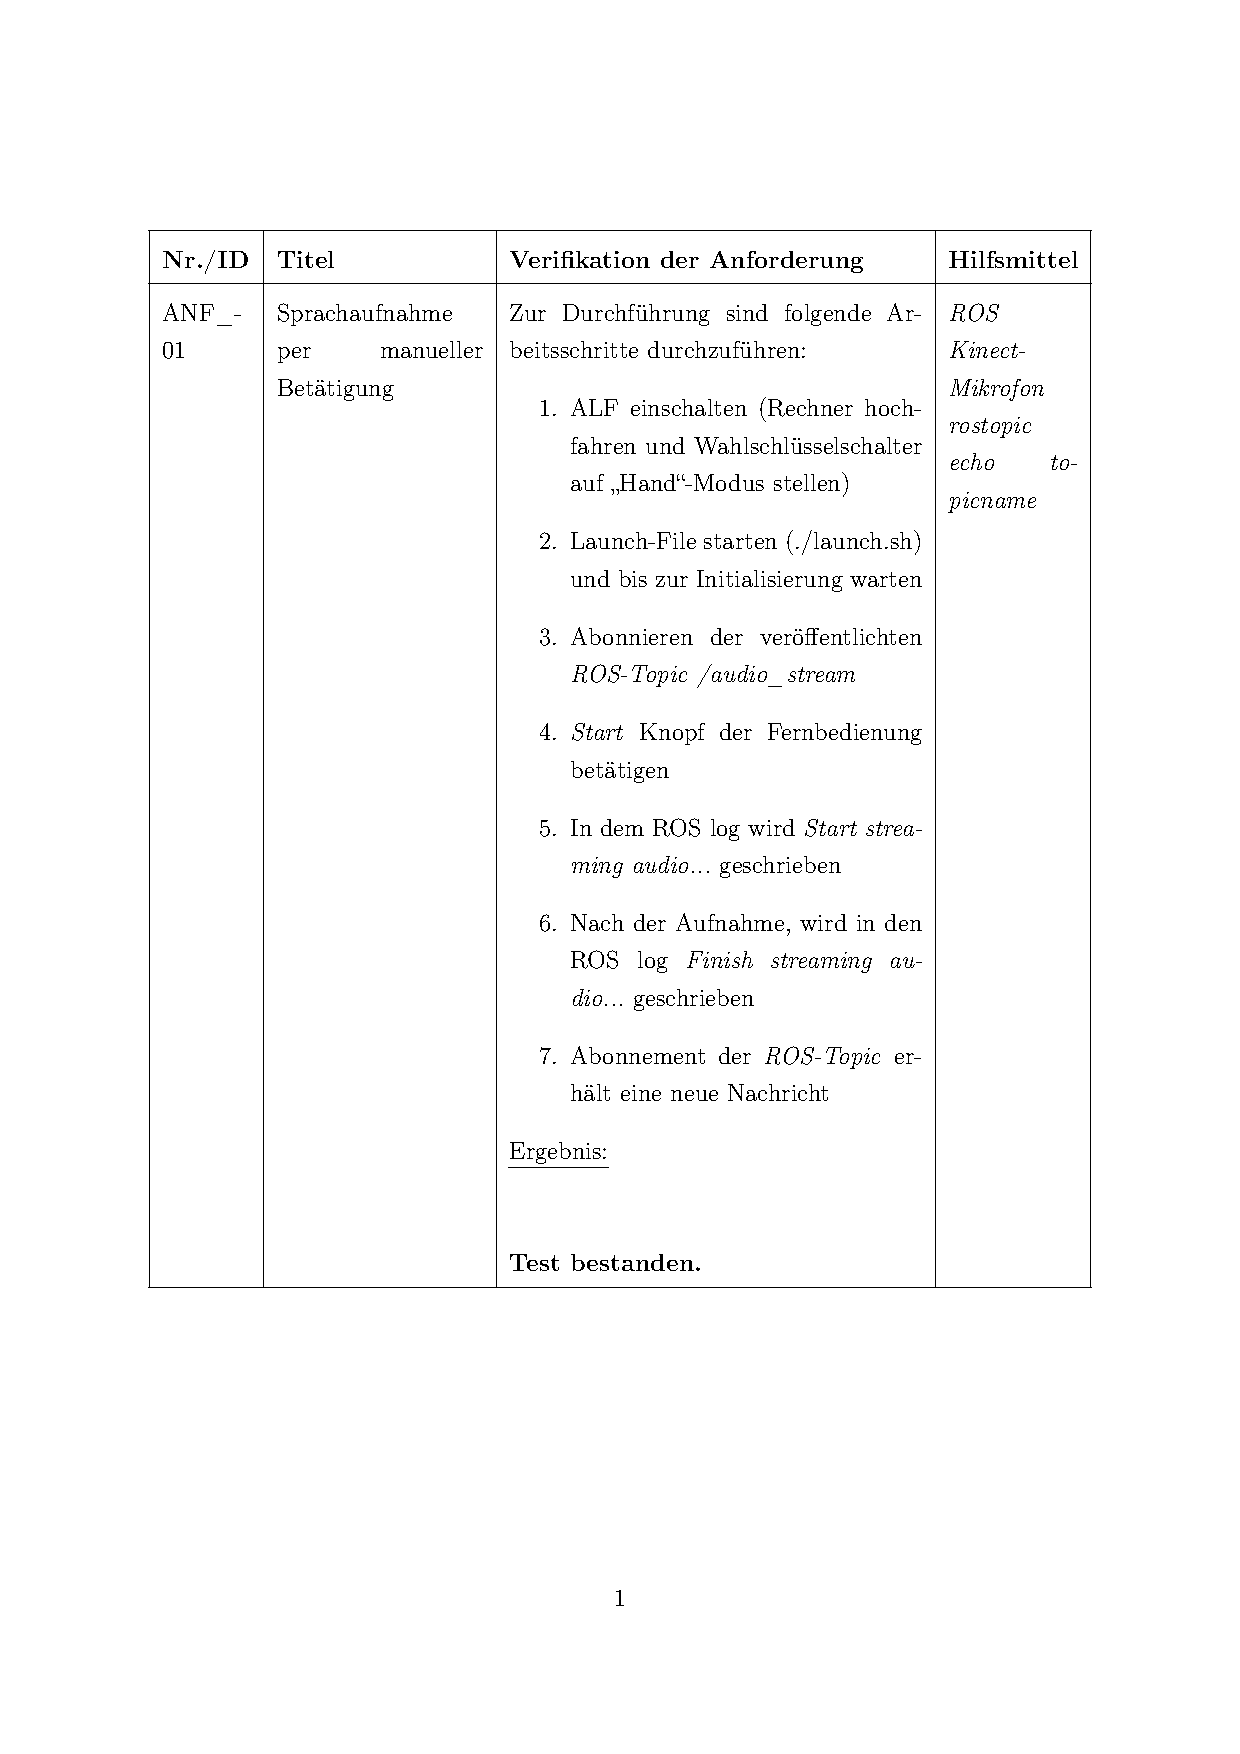
\includegraphics[width=1.0\textwidth]{Bilder/Verifikationsplan.png} 
	\caption{Verifikationsplan}
	\label{fig:Verlängerung der Welle mit Bremskegel}
	%\caption*{Quelle: Eigene Darstellung}
\end{figure}

\chapter{Ausblick und Fazit}
\label{chap:Ausblick und Fazit}

Anhand der Laborversuche zeigte sich, dass das Motorverhalten nicht dem einer handelsüblichen Synchronmaschine entspricht. Dies hat keine Auswirkungen auf den Polradwinkel sondern beschreibt untypisches Verhalten der Strangspannung und -ströme unter Last. Daraus folgt, dass die Rotorposition im Rahmen dieses Entwicklungsprojekts nur mit einem induktiven Sensor bestimmt werden konnte. Es stellte sich heraus, dass eine Verifikationen der Ergebnisse anhand einer Fourier-Analyse oder einem Zeigerbild problematisch ist. Die in diesem Entwicklungsprojekt konzipierte Methode den Polradwinkel zu messen, kann an allen möglichen Synchronmaschinen genutzt werden.

Es sind verschiedene Erweiterungen des Syngle-Moduls denkbar:

	\begin{itemize}
	\item Bisher wurde das Erfassen des Polradwinkels lediglich an dem UniTrain System durchgeführt. Die Messung des Polradwinkels mit der entwickelten Methode an einem handelsüblichen Motor kann mit entsprechenden Anpassungen durchgeführt werden
	\item Konstruktion des Syngle-Moduls als eingebettetes System, welches keinen externen Rechner mehr benötigt. Möglich wäre ein von National Instruments unanhängiger Microcontroller, auf welchem per Model Based Design eine Software Architektur implementiert werden kann, z.B. mithilfe von Matlab/Simulink.
	\item Erfassen des Polradwinkels an handelsüblichen Maschinen anhand der vorliegenden elektrischen Größen, statt die Rotorposition (siehe Kapitel 3.3.3) mit einem induktiven Sensor zu bestimmen.
\end{itemize}


%%% Local Variables: 
%%% mode: latex
%%% TeX-master: "main"
%%% TeX-open-quote: "\\enquote{"
%%% TeX-close-quote: "}"
%%% LaTeX-csquotes-open-quote: "\\enquote{"
%%% LaTeX-csquotes-close-quote: "}"
%%% End: 